% This is a basic Math Paper

\documentclass[11pt]{article}

% Preamble

\usepackage[margin=1in]{geometry}
\usepackage{amsfonts, amsmath, amssymb}
\usepackage{fancyhdr, float, graphicx}
\usepackage[utf8]{inputenc} % Required for inputting international characters
\usepackage[T1]{fontenc} % Output font encoding for international characters
\usepackage{fouriernc} % Use the New Century Schoolbook font
\usepackage[nottoc, notlot, notlof]{tocbibind}
\usepackage[hidelinks]{hyperref}

% Header and Footer
\pagestyle{fancy}
\fancyhead{}
\fancyfoot{}
\fancyhead[L]{\textit{\Large{Robot-Assisted Automatic Conveyor System}}}
%\fancyhead[R]{\textit{something}}
\fancyfoot[C]{\thepage}
\renewcommand{\footrulewidth}{1pt}



% Other Doc Editing
% \parindent 0ex
%\renewcommand{\baselinestretch}{1.5}

\begin{document}
	
	\begin{titlepage} 
		\centering 
		
		%---------------------------NAMES-------------------------------
		
		\huge\textsc{
			MIT World Peace University
		}\\
	
		\vspace{0.75\baselineskip} % space after Uni Name
		
		\LARGE{
			Basic Mechanical Engineering\\
			First Year B. Tech, Trimester 1
		}
		
		\vfill % space after Sub Name
		
		%--------------------------TITLE-------------------------------
		
		\rule{\textwidth}{1.6pt}\vspace*{-\baselineskip}\vspace*{2pt}
		\rule{\textwidth}{0.6pt}
		\vspace{0.75\baselineskip} % Whitespace above the title
		
		
		
		\huge{\textsc{
				Demonstration of Robot-Assisted Automatic Conveyor System
			}} \\
		
		
		
		\vspace{0.5\baselineskip} % Whitespace below the title
		\rule{\textwidth}{0.6pt}\vspace*{-\baselineskip}\vspace*{2.8pt}
		\rule{\textwidth}{1.6pt}
		
		\vspace{1\baselineskip} % Whitespace after the title block

		%--------------------------SUBTITLE --------------------------	
			
		\LARGE\textsc{
			Experiment Number 5\\Practical Report
		} % Subtitle or further description
		\vfill
		
		%--------------------------AUTHOR-------------------------------
		
		Prepared By
		\vspace{0.5\baselineskip} % Whitespace before the editors
		
		\Large{
			Krishnaraj Thadesar \\
			Division 9, Roll No. 54
		}
		
		
		\vspace{0.5\baselineskip} % Whitespace below the editor list
		\today

	\end{titlepage}
	
	
\tableofcontents
\thispagestyle{empty}
\clearpage


\setcounter{page}{1}

\section{Objective}
To study Conveyor Systems and Robot Assisted Material Systems


\section{Theory}


A conveyor system is a common piece of mechanical handling equipment that moves
materials from one location to another. Conveyors are especially useful in applications involving the transport of heavy or bulky material. Conveyor systems allow quick and efficient transport for a wide variety of material, which make them very popular in the material handling and packaging industries.\\

They also have popular consumer applications, as they are often found in supermarkets and airports, constituting the final leg of item/ bag delivery to customers. Many kinds of conveying systems are available and are used according to the various needs of different industries.\\ 
There are chain conveyors (floor and overhead) as well. Chain conveyors consist of enclosed tracks, I-Beam, towline, powered and free hand pushed trolleys etc.

Eg. Roller conveyor for carton transport in the apparel industry

\subsection{Advantages of Conveyor Systems}

Conveyor systems are used widespread across a range of industries due to the numerous benefits they provide.

\begin{enumerate}
	\item Conveyors are able to safely transport materials from one level to another, which when done by humans, labor would be strenuous and expensive.
	\item They can be installed almost anywhere, and are much safer than using a forklift or other machine to move materials.
	\item They can be installed almost anywhere, and are much safer than using a forklift or other machine to move materials.
	\item There are a variety of options available for running conveying systems, including the hydraulic, mechanical and fully automated systems, which are equipped to fit individual needs.
\end{enumerate}

\subsection{Design and Selection of Conveyor Systems}

Conveyors can be linked together with other machinery to become an integral component of a processing or packaging line. \\
The best way to accomplish this is to consider following variables to envisage how the conveyors should interact with the assembly line they are integrating with:

\begin{enumerate}
	\item What are the goals and objectives for processing/assembly line?
	\item What is the products that need to be moved?
	\item What is the weight, size and packaging of the products?
	\item What is the rate of production for the application (desired speed of the conveyors)?
	\item How are the conveyors going to integrate with other equipment/machinery on the line?
	\item Are there any product transfers involved?
	\item What is the projected product flow of the application (sorting, accumulation, curves, inclines, declines etc.)?
	\item What type of environment will the conveyor be operating in? If it will require cleaning, how extensive does that cleaning need to be?
	\item Will robotics be integrated with the conveyor system?
\end{enumerate}


All components within an assembly automation application, including conveyors, should work together to best augment the overall operation. Answering those questions will help to take a critical look at the conveyor system to determine where improvements in product flow and handling can be made.

\subsection{Industry Application}

Conveyor systems are commonly used in many industries, including the Mining, automotive,
agricultural, computer, electronic, food processing, aerospace, pharmaceutical, chemical, bottling and canning, print finishing and packaging. Although a wide variety of materials can be conveyed, some of the most common include food items such as beans and nuts, bottles and cans, automotive components, scrap metal, pills and powders, wood and furniture and grain and animal feed. \\

Many factors are important in the accurate selection of a conveyor system. It is important to know how the conveyor system will be used beforehand. Some individual areas that are helpful to consider are the required conveyor operations, such as transport, accumulation and sorting, the material sizes, weights and shapes and where the loading and pickup points need to be. Conveyors are built to required specifications to improve efficiency and output of production line.


\subsection{Latest Trends in Conveyor Systems}

\begin{enumerate}
	\item \textit{Conveyors for Flexible Assembly lines}: Modern production facilities show a growing trend of flexible assembly lines. Assembly lines need to be flexible to accommodate different applications. The supporting conveyor system needs to be just as flexible. Modular conveyors are mobile and can be easily moved from one line to another. The conveyor’s guiding, transfers and other accessories may need to be adjusted.
	\item \textit{Conveyors are continuing to play a greater role in robotic applications.} Robotic movements are 	precise and exact – conveyors need to operate to that same level of accuracy. Robotic applications often require product to be in an exact spot on the conveyor at the right time. But to do that successfully	requires a conveyor system that’s efficient, reliable and engineered to work in conjunction with robotics. Servo motor precision move conveyors deliver accurate alignment of time and distance that provide indexing repeatability of +/- .040”, all at a rate of 100 indexes per minute. It’s important to select a conveyor to perfectly match the application requirements.
	
\end{enumerate}

\pagebreak

\subsection{Robotic Material Handling and Tending}


Robotic material handling and tending systems are commonplace in the industrial sector. Material handling refers to robotic arms moving production parts, typically on or off a conveyor belt or to hold a part in place for production. Machine tending is similar, but more specific, referring to a robotic arm to load and unload a stationary production machine.\\
Both robotic material handling and machine tending systems are in high demand as they reliably deliver productivity gains in a wide range of applications.\\

\subsubsection{The Benefits of Robotic Material Handling and Machine Tending Systems}
Much of the benefits of these systems comes from drastically increased uptime. Manual material handling and tending is slow, inconsistent and less productive. Robots can work around the clock, besides small periods of downtime for maintenance, with high levels of consistency. \\

In addition to increased up-time, robots are typically much faster than manual processes. Decreasing the cycle time of a production part impacts productivity in a positive way. The benefit of shorter cycle times compounds over time and are extremely valuable to manufacturers.


\section{Application of Conveyor Systems in Smartphone Manufacturing Process}

The Smartphone Industry is heavily dependent on Robotic assistance in Manufacturing. The parts that need to be assembled are intricate, small and need precise placement. These reasons make it essential for manufactures to go with Robotic Arms (see fig:\ref{fig:Robotic Arms}) and Conveyor belts for mass production. 


\begin{figure}[H]
	\centering
	\includegraphics[scale=0.3]{Robotic Arms.jpg}
	\caption{Robotic Arms handling a Smartphone Body\cite{How Smartphones Are Made in Factory}}
	\label{fig:Robotic Arms}
\end{figure}

\pagebreak
While delicate parts are handled by the Robotic Arms, the chipsets and electronics are usually transported using specialized conveyor belts operated by motors (see fig:\ref{fig:Conveyors for chipsets})


\begin{figure}[H]
	\centering
	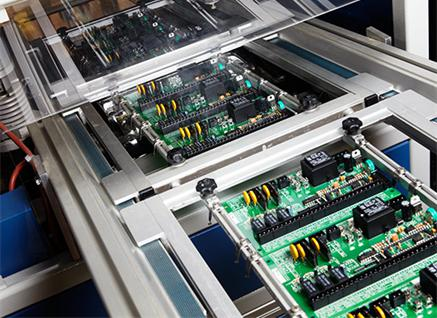
\includegraphics[scale=0.7]{Conveyors in Smartphones.jpg}
	\caption{Motorized conveyors transporting a Chipset\cite{How Smartphones Are Made | Smartphone Factory Tour}}
	\label{fig:Conveyors for chipsets}
\end{figure}


\subsection{Advantages}

\begin{enumerate}
	\item The right conveyor control saves time, money and efficiency. It will optimize your material handling systems and warehouse operations. 
	\item It will allow for variable production rates and quick production changes. Programmable Logic Controls (PLC) allow for this necessary direct system control. 
	\item This centralized network-oriented approach is best primed for automation and attaining the numbers you need to thrive.
	
\end{enumerate}

\subsection{The Belt Conveyor}

\subsubsection{Definition}
A conveyor belt is the carrying medium of a belt conveyor system (often shortened to \textit{belt conveyor}). A belt conveyor system is one of many types of conveyor systems. A belt conveyor system consists of two or more pulleys (sometimes referred to as drums), with a closed loop of carrying medium—the conveyor belt—that rotates about them. One or both of the pulleys are powered, moving the belt and the material on the belt forward. The powered pulley is called the drive pulley while the unpowered pulley is called the idler pulley.\\
 
They are used widely to transport Electronic and outer Body parts of the Smartphone from one Machine in the Factory to another. (see fig:\ref{fig:Belt Conveyors})


\begin{figure}[H]
	\centering 
	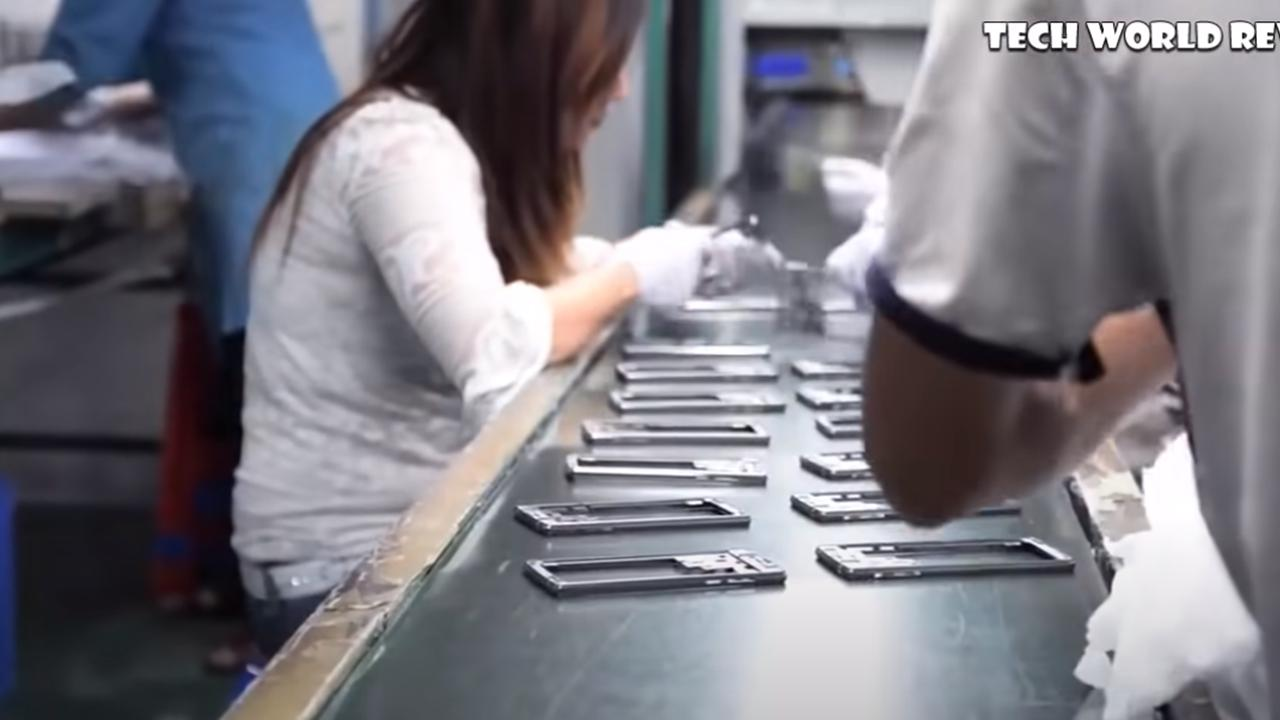
\includegraphics[scale=0.3]{Belt conveyors.jpg}
	\caption{Belt Conveyors being used to transport Parts\cite{How Smartphones are made in China}}
	\label{fig:Belt Conveyors}
\end{figure}




\subsubsection{Merits and Demerits}
Here are some of the most common advantages and disadvantages of Belt conveyors.\\


\textbf{Merits:}
\begin{enumerate}
	\item One of the cheapest conveyors
	\item Simple and easy to use
	\item Can have changes in elevation
	\item Can be loaded from any place along the belt\\
\end{enumerate}


\textbf{Demerits:}
\begin{enumerate}
	\item The Simplicity means very limited features
	\item Belt can be difficult to clean and generally does not leave a very successful result
	\item Sticky material can get stuck on the belt and terasfer to the return side, the rolls, idlers and pulleys. 
\end{enumerate}


\section{Conclusion}
	
The Working, Advantages, and disadvantages of Robot Assisted Automatic Conveyor Systems were studied and understood. Their application in the Smartphone Manufacturing Process was seen in depth, and their Significance in each such industry was emphasized. \\
\textit{While they can be an investment on the side of the Manufactures, their merits far exceed their demerits in large scale Industry Applications.}



\pagebreak
\begin{thebibliography}{}


\bibitem{How Smartphones Are Made in Factory}
"How Smartphones Are Made in Factory"\\
\url{https://www.youtube.com/watch?v=psDO1rPFQ1Y}\\
Image taken from this You-Tube Video.
	
\bibitem{How Smartphones Are Made | Smartphone Factory Tour}
"How Smartphones Are Made | Smartphone Factory Tour"\\
\url{https://www.youtube.com/watch?v=t_mgrSd9fdY}\\
Image taken from this You-Tube Video.

\bibitem{How Smartphones are made in China}
"How Smartphones are made in China"\\
\url{https://www.youtube.com/watch?v=nCPNH5QzEB8&t=156s}\\
Image taken from this You-Tube Video.

	
	
\end{thebibliography}
	
	
\end{document}